\section{Auswertung}

Ausgleichsrechnungen mit Fehlerfortpflanzung werden mit scipy.optimize.curve\_fit \cite{scipy}
aus dem Programm Python durchgeführt.

\subsection{Kontrast}

Der Kontrast gibt das Verhältnis zwischen dem Intensitätsminimum und -maximum an, vgl. Gleichung
\ref{kontra}. Ein Fit nach der Gleichung für den Kontrast
\[
K = a \cdot | \sin (2 \cdot \phi + b) |
\]
liefert die Fitparameter $a = 1.06 \pm 0.05$ und $b = 1 \pm 2$. Ein Plot der Messwerte und der
Ausgleichsrechnung sind in Abbildung \ref{kontrast} zu sehen. Die Messwerte sind zudem in Tabelle
zusammengefasst.

\begin{figure}[h]
\centering
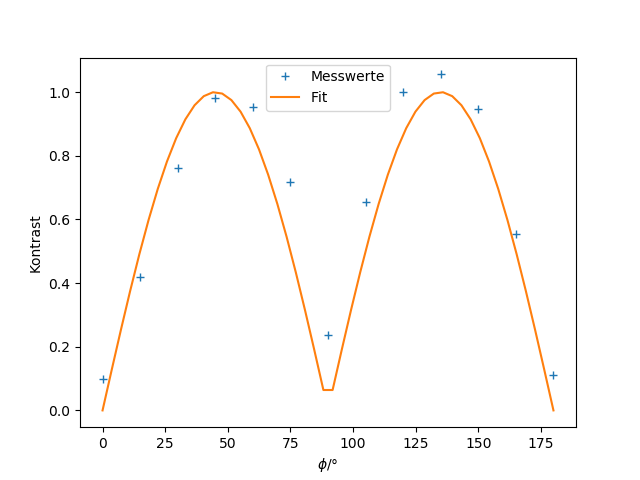
\includegraphics[width=\linewidth]{img/kontrast.png}
\caption{Ausgleichsrechnung für den Zusammenhang zwischen dem Winkel $\phi$ und dem Kontrast $K$.}
\label{kontrast}
\end{figure}

\begin{table}
  \caption{Messwerte für $I_\text{min}$ und $I_\text{max}$ bei dem Winkel $\phi$.}
  \label{tab:glas}
  \centering
  \begin{tabular}{c|c|c}
    $\phi$/° & $V_\text{max}$/mV & $V_\text{min}$/mV \\ \midrule
    0 & -287.5  & -350.0 \\
    15 & -212.5 &  -518.8 \\
    30  & -87.5 & -650.0 \\
    45  & -6.25 & -668.8 \\
    60  & -12.5 & -537.5 \\
    75  & -56.25  & -343.8 \\
    90  & -100.0  & -162.5 \\
    105 & -31.25  & -150.0 \\
    120 & 0.0 & -162.5 \\
    135 & 6.25  & -231.2 \\
    150 & -8.75 & -325.0 \\
    165 & -112.5  & -393.8 \\
    180 & -300.0  & -375.0 \\
  \end{tabular}
\end{table}

\subsection{Brechungsindex von Glas}

Die Ausgleichsrechnung nach der Funktion in Gleichung (\ref{glas})
liefert den Fitparameter $a = 1.553 \pm 0.009$, was auch bereits der Brechungsindex von Glas ist.
Der lineare zwischen dem Winkel $\theta$ der Anzahl der Intensitätsmaxima mit dem Brechungsindex $n$
als Steigung ist zusammen mit den gemessenen Werten in Abbildung dargestellt. In Tabelle \ref{tab:glas}
sind die dazugehörigen Messwerte zu sehen.

\begin{figure}[h]
\centering
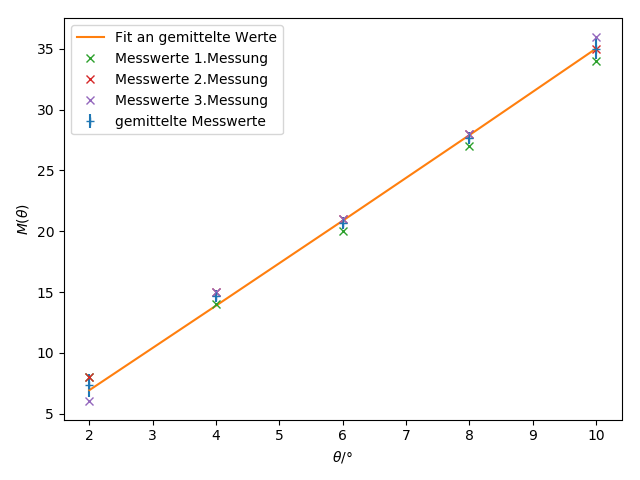
\includegraphics[width=\linewidth]{img/n_glas.png}
\caption{Lineare Ausgleichsrechnung für den Zusammenhang zwischen dem Winkel $\theta$ und der Anzahl
der Intensitätsmaxima.}
\label{n_glas}
\end{figure}

\begin{table}
  \caption{Messwerte für den Zusammenhang zwischen dem Winkel $\theta$ und der Anzahl
  der Intensitätsmaxima.}
  \label{tab:glas}
  \centering
  \begin{tabular}{c|c|c|c}
    $\theta/°$ & $M_1$ & $M_2$ & $M_3$ \\ \midrule
    2 & 8 & 8 & 6 \\
    4 & 14  & 15  & 15 \\
    6 & 20  & 21  & 21 \\
    8 & 27  & 28  & 28 \\
    10 & 34 & 35  & 36
  \end{tabular}
\end{table}

\subsection{Brechungsindex von Luft}

In Anlehnung an Gleichung \ref{n_gas} wird ein Fit der Form
\[
n = \sqrt{a \cdot p + 1}
\]
mit $a = \sfrac{3A}{RT}$ durchgeführt. Dieser liefert den Fitparameter
$a = 6.05 \cdot 10^{-7} \pm 0.04 \cdot 10^{-7}$. Dieser Faktor wird mit der gemessenen Temperatur
$T = \SI{22.2}{\degreeCelsius}$ auf Normaltemperatur $T_0 = \SI{15}{\degreeCelsius}$ skaliert.
Daraus ergibt sich mit dem Normaldruck $p_0 = \SI{1013}{\milli\bar}$ der Brechungsindex von Luft bei
Normalbedingungen nach
\[
n = \sqrt{1 + a \cdot \frac{T}{T_0} \cdot p_0} = 1.000453 \pm 0.000003.
\]
bestimmt. Die entsprechenden Messwerte sind in Tabelle \ref{tab:luft} die Ausgleichsrechnung wird
in Abbildung \ref{n_luft} gezeigt. Die letzten fünf Werte konnten bei der 3. Messung nicht aufgenommen
werden, da der Zähler auf einen Wert >60 gesprungen ist. Sie wurden

\begin{figure}[h]
\centering
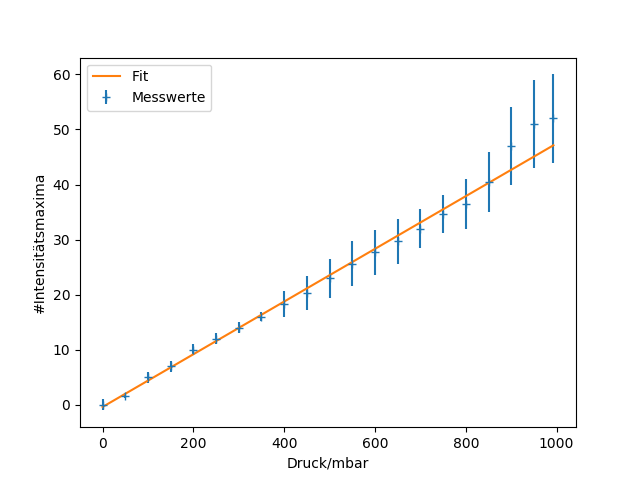
\includegraphics[width=\linewidth]{img/n_luft.png}
\caption{Lineare Ausgleichsrechnung für den Zusammenhang zwischen dem Druck $p$ und dem Brechungsindex.}
\label{n_luft}
\end{figure}

\begin{table}
  \caption{Messwerte für den Zusammenhang zwischen dem Druck $p$ und der Anzahl
  der Intensitätsmaxima.}
  \label{tab:luft}
  \centering
  \begin{tabular}{c|c|c|c}
    $p$/mbar &  $M_1$ & $M_2$ & $M_3$ \\ \midrule
    0 & 0 & 0 & 0 \\
    50 & 1 & 2 & 2 \\
    100 & 5 & 5 & 5 \\
    150 & 7 & 7 & 7 \\
    200 & 10  & 10  & 10 \\
    250 & 12  & 12  & 12 \\
    300 & 14  & 14  & 14 \\
    350 & 15  & 17  & 16 \\
    400 & 15  & 20  & 20 \\
    450 & 16  & 23  & 22 \\
    500 & 18  & 25  & 26 \\
    550 & 20  & 28  & 29 \\
    600 & 22  & 30  & 31 \\
    650 & 24  & 32  & 33 \\
    700 & 27  & 34  & 35 \\
    750 & 30  & 36  & 38 \\
    800 & 32  & 41  & - \\
    850 & 35  & 46  & - \\
    900 & 40  & 54  & - \\
    950 & 43  & 59  & - \\
    993 & 44  & 60  & - \\
  \end{tabular}
\end{table}
